\documentclass[12pt,letterpaper]{exam}
\usepackage[lmargin=1in,rmargin=1in,tmargin=1in,bmargin=1in]{geometry}
\usepackage{../style/exams}

% -------------------
% Course & Exam Information
% -------------------
\newcommand{\course}{MAT 101: Exam 2}
\newcommand{\term}{Winter -- 2021}
\newcommand{\examdate}{01/14/2021}
\newcommand{\timelimit}{95 Minutes}

\setbool{hideans}{true} % Student: True; Instructor: False

% -------------------
% Content
% -------------------
\begin{document}

\examtitle
\instructions{Write your name on the appropriate line on the exam cover sheet. This exam contains \numpages\ pages (including this cover page) and \numquestions\ questions. Check that you have every page of the exam. Answer the questions in the spaces provided on the question sheets. Be sure to answer every part of each question and show all your work.} 
\scores
\bottomline
\newpage

% ---------
% Questions
% ---------
\begin{questions}

% Question 1
\newpage
\question[6] A table of values for a function $f(x)$ is given below.
	\begin{table}[!ht]
	\centering
	\begin{tabular}{r||rrrrrrrrrrr}
	$x$ & $-5$ & $-4$ & $-3$ & $-2$ & $-1$ & $0$ & $1$ & $2$ & $3$ & $4$ & $5$ \\ \hline
	$f(x)$ & $6$ & $3$ & $0$ & $-2$ & $4$ & $6$ & $3$ & $0$ & $5$ & $6$ & $8$
	\end{tabular}
	\end{table} \par
Determine the $y$-intercepts and $x$-intercepts for the function $f(x)$. \pspace



\newpage



% Question 2
\newpage
\question[6] A table of values for a function $f(x)$ is given below. Determine whether the function $f(x)$ is linear or not. Be sure to fully justify your answer. \par
	\begin{table}[!ht]
	\centering
	\begin{tabular}{r||rrrrrrrrrrr}
	$x$ & $0$ & $1$ & $2$ & $4$ & $5$ & $6$ \\ \hline
	$f(x)$ & $-5$ & $-2$ & $1$ & $7$ & $11$ & $13$
	\end{tabular}
	\end{table} \pspace



\newpage



% Question 3
\newpage
\question[4] Sketch the line $3x - 5y= 10$ on the plot below. 
	\[
	\fbox{
	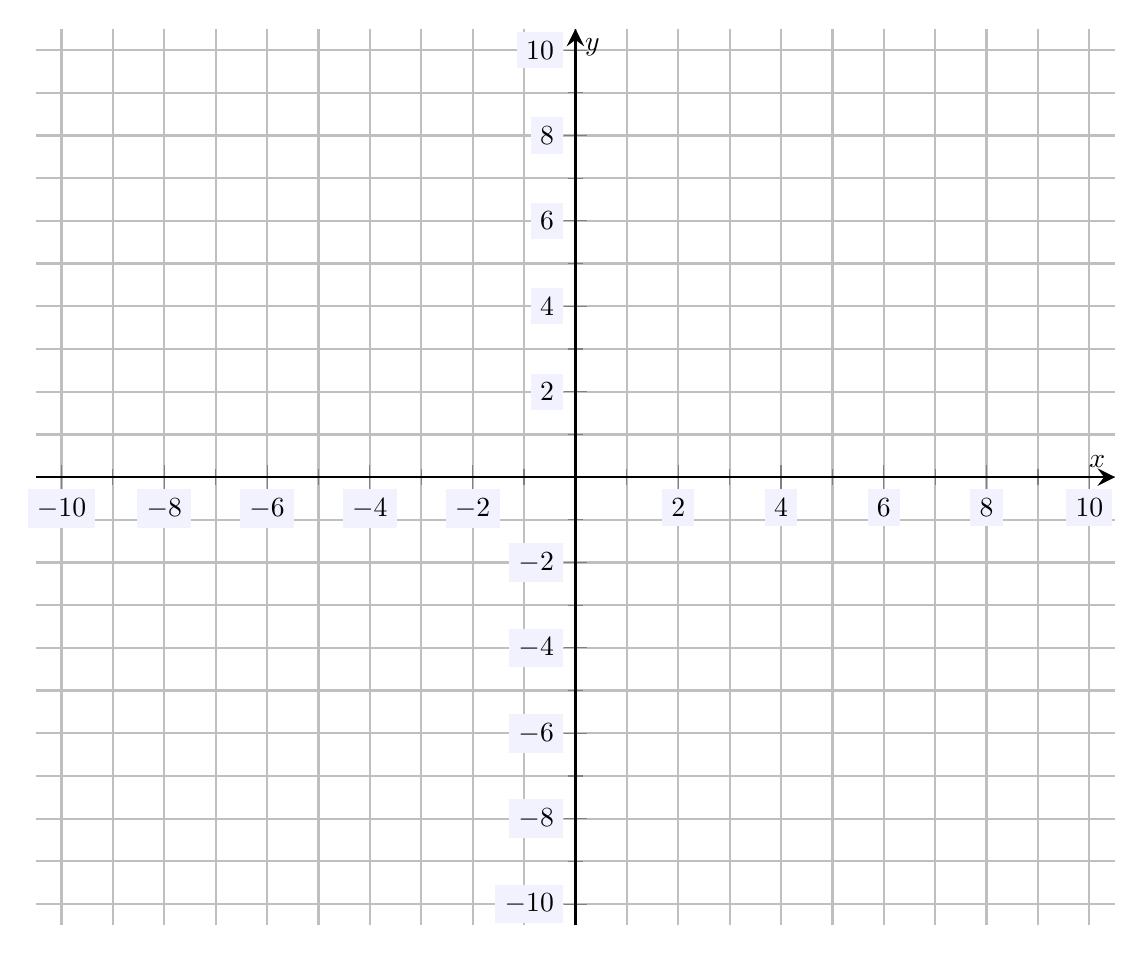
\begin{tikzpicture}[scale=2,every node/.style={scale=0.5}]
	\begin{axis}[
	grid=both,
	axis lines=middle,
	ticklabel style={fill=blue!5!white},
	xmin= -10.5, xmax=10.5,
	ymin= -10.5, ymax=10.5,
	xtick={-10,-8,-6,-4,-2,0,2,4,6,8,10},
	ytick={-10,-8,-6,-4,-2,0,2,4,6,8,10},
	minor tick = {-10,-9,...,10},
	xlabel=\(x\),ylabel=\(y\),
	]
	\end{axis}
	\end{tikzpicture}
	}
	\] \pspace



\newpage



% Question 4
\newpage
\question[6] Two lines are given below. Determine whether these lines are the same or parallel. Determine also whether these lines intersect or not. If so, determine whether they intersect perpendicularly. 
	\[
	\begin{aligned}
	\ell_1&: & y&= 8 - \dfrac{5}{6}\,x \\
	\ell_2&: & 6x &+ 5y= 15
	\end{aligned}
	\] \pspace



\newpage



% Question 5
\newpage
\question[6] A table of values for a linear function $f(x)$ is given below.
	\begin{table}[!ht]
	\centering
	\begin{tabular}{r||rrrrrrrrrrr}
	$x$ & $-12$ & $-8$ & $-4$ & $\phantom{-}4$ & $\phantom{-}8$ & $\phantom{-}12$ \\ \hline
	$f(x)$ & $21$ & $18$ & $15$ & $9$ & $6$ & $3$
	\end{tabular}
	\end{table} \par
Determine the equation for $f(x)$. \pspace



\newpage



% Question 6
\newpage
\question[6] Find the equation of the line that contains the points $(-10, 15)$ and $(2, -1)$. \pspace



\newpage



% Question 7
\newpage
\question[6] Determine the equation of the line that contains the point $(6, 10)$ and is perpendicular to the line $y= -1$. \pspace 



\newpage



% Question 8
\newpage
\question[6] Find the equation of the line that is perpendicular to the line $y= 4 - 5x$ and passes through the $y$-intercept of the line $y= 2x + 3$. \pspace



\newpage



% Question 9
\newpage
\question[6] A researcher creates a model to predict adolescent male's weight (in lbs) from their height (in cm). The model is $W(h)= 2.6h - 17.3$.
	\begin{enumerate}[(a)]
	\item Is the model linear? Explain.
	\item Determine the slope of $W(h)$. Interpret the slope in context.
	\item Determine the $y$-intercept of $W(h)$. Does the $y$-intercept have meaning in this context? Explain.
	\end{enumerate} \pspace



\newpage



% Question 10
\newpage
\question[4] Sketch the function $f(x)= 8 - (x + 3)^2$ on the plot below. 
	\[
	\fbox{
	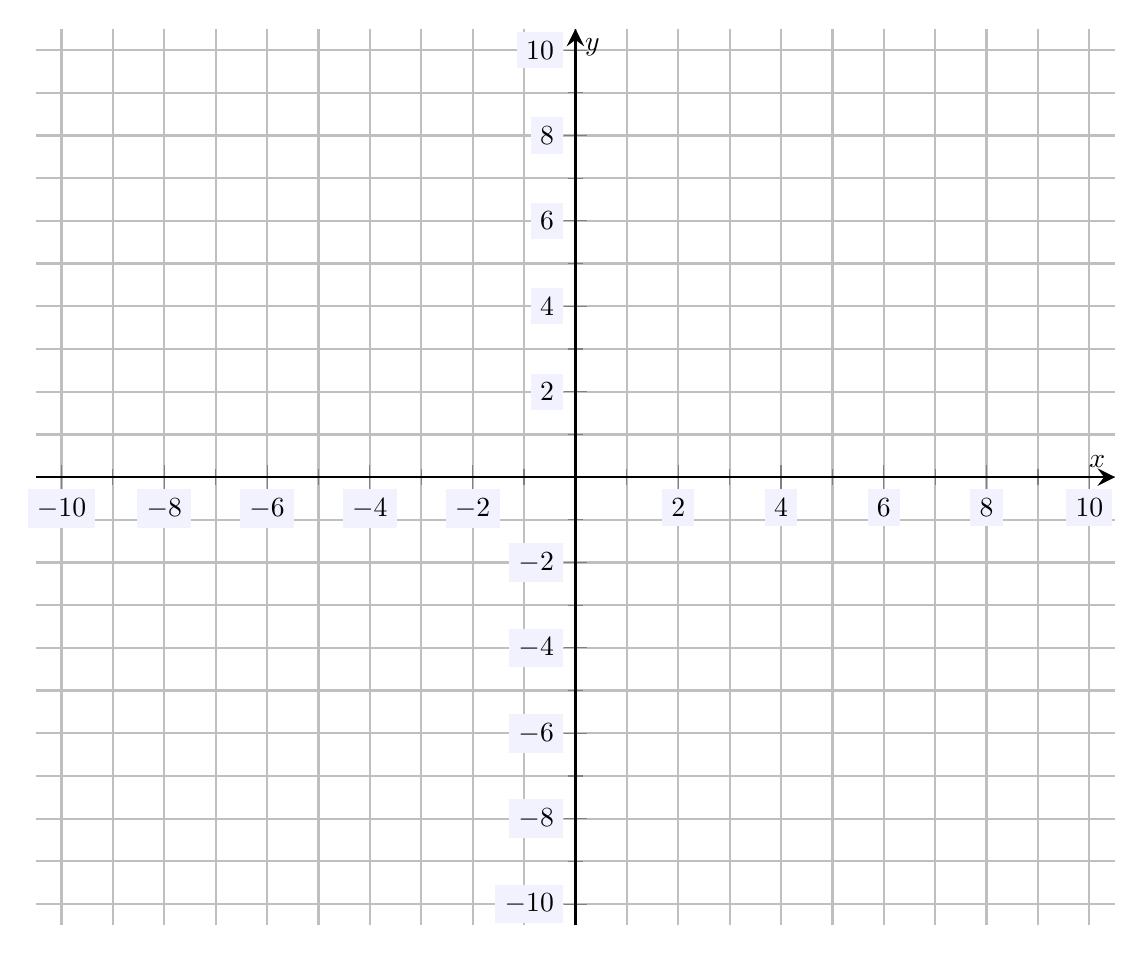
\begin{tikzpicture}[scale=2,every node/.style={scale=0.5}]
	\begin{axis}[
	grid=both,
	axis lines=middle,
	ticklabel style={fill=blue!5!white},
	xmin= -10.5, xmax=10.5,
	ymin= -10.5, ymax=10.5,
	xtick={-10,-8,-6,-4,-2,0,2,4,6,8,10},
	ytick={-10,-8,-6,-4,-2,0,2,4,6,8,10},
	minor tick = {-10,-9,...,10},
	xlabel=\(x\),ylabel=\(y\),
	]
	\end{axis}
	\end{tikzpicture}
	}
	\] \pspace



\newpage



% Question 11
\newpage
\question[6] Showing all your work, find the vertex form of $y= 2x^2 - 12x + 23$. \pspace



\newpage



% Question 12
\newpage
\question[6] Showing all your work, factor the polynomial $x^2 - 22x - 48$. \pspace



\newpage



% Question 13
\newpage
\question[6] Showing all your work, factor the polynomial $5x^2 + 19x - 4$. \pspace



\newpage



% Question 14
\newpage
\question[6] Showing all your work, solve the equation $2x= 24 - x^2$. \pspace



\newpage



% Question 15
\newpage
\question[6] Showing all your work, use the quadratic equation to solve $2x^2= 4x - 10$. \pspace



\newpage



% Question 16
\newpage
\question[4] Consider the quadratic function $f(x)= x^2 - 6x + 4$. Use the discriminant of $f(x)$ to show that $f(x)$ does not factor `nicely', then use the quadratic formula to factor $f(x)$. \pspace



\newpage



% Question 17
\newpage
\question[10] Consider the function $f(x)= 3x^2 - 15x + 20$. 
	\begin{enumerate}[(a)]
	\item Determine if the parabola is concave up or concave down. 
	\item Determine the axis of symmetry of $f(x)$. 
	\item Determine the vertex of $f(x)$.
	\item Does $f(x)$ have a maximum or minimum value? Explain. 
	\item Find the maximum or minimum value of $f(x)$ from (d).  
	\end{enumerate}


\end{questions}
\end{document}